\chapter{Project Plan}
This section is an excerpt of the project plan. The project plan features descriptions of which experiments, technologies etc. to conduct, investigate and implement during the Bachelor's Project. \newline

This section contains how the project work will be structured, which methods to be used, etc. \newline

\subsection{The Bachelor's Project}
The Bachelor’s Project (Thesis or Final Project) is an extensive project dealing with a realistic engineering assignment. The bachelor project should document the students’ ability to work independently to apply engineering methods and theories in solving professional problems and development issues in a specific field. The project constitutes the conclusion of the programme and is placed in the last semester. \newline

The Bachelor's Project workload is \textbf{20 ECTS points}. \textbf{1 ECTS} translates to \textbf{27 hours of workload}, totaling \textbf{540 hours} of workload for the Bachelor's Project. Assuming 18 weeks of Bachelor's Project work, total workload/week is ~30 hours/week. \newline

During the project period, 2 elective courses with 10 ECTS points in total to fulfill the goal of 30 ECTS workload each semester. Assuming 18 weeks of lectures and homework assignments and projects, total workload/week is ~16-17 hours/week. \newline

Total workload is therefore expected to be ~45-50 hours/week during the semester. To keep track of the project, weekly SCRUM meetings with supervisor is essential along with project management tools: \\

- The ASE-model \\
- SCRUM \\
- Redmine \newline

\subsection{ASE-model}

\begin{figure}[H]
\centering
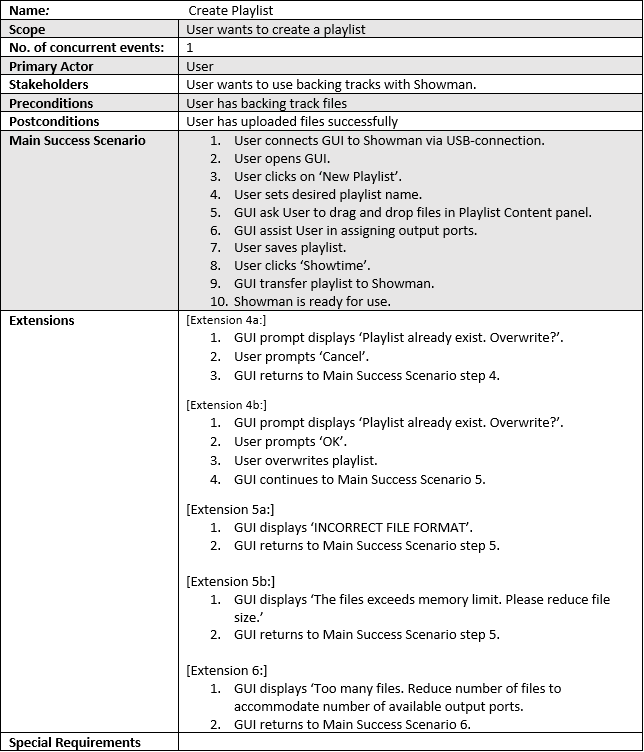
\includegraphics[scale=1]{./pictures/UC1.png}
\caption{Use-Case diagram of Use-Case 1.}
\label{fig:UC1.png}
\end{figure}

\subsection{SCRUM}
An agile project development management is used in this pro


\subsection{Redmine}


\subsection{Supervisor Meetings}


\subsection{Timetable}


%\textbf{Objective} \\
%The objective of the Bachelor’s Project is that students be able to plan and conduct an engineering project in as realistic a form as the study environment allows, preferably in cooperation with companies. \\

%\textbf{Learning Objectives} \\
%Upon completion of the Bachelor’s Project, the student should be able to: \\

%- Apply scientific research results and technological knowledge for solving  technical problems, \\
%- Develop new solutions, \\
%- Acquire and evaluate new knowledge within relevant engineering fields, \\
%- Systematically apply engineering knowledge, theories and methods \\
%- Plan and complete a project in a group in cooperation with internal and external partners \\
%- Present results of a project in writing and orally by means of relevant communication tools, to professionals as well as customers, \\
%- Present results of a project orally and with means of various audio or visual communication tools, \\
%- Integrate social, economic, environmental and work environmental consequences in the solution model \newline

%Learning objectives in relation to the specific subject and with reference to above, including their weight, is specified in the Assignment Formulation. \newline

%\textbf{Main Content} \\
%The Bachelor’s Project should comprise the planning and documentation of solutions for a realistic engineering project or defined parts and comprise independent experimental, empirical and/or theoretical discussions and computations. \\

%\subsection{Project Plan}
%Project management tools are needed for the project to keep focus. Aarhus School of Engineering development model 